\begin{example}
    \begin{figure}
        \centering
        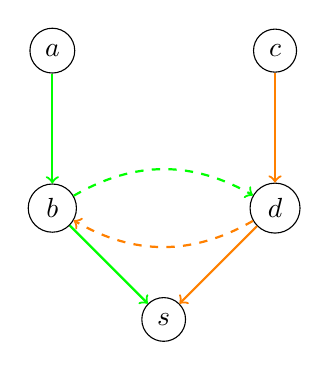
\begin{tikzpicture}[
                node distance={20mm},
                main/.style = {draw, circle},
                s/.style = {->,thick},
                d/.style = {->,thick,dashed} ]
            \node[main] (s) {$s$};
            \node[main] (b) [above left of=s] {$b$};
            \node[main] (a) [above of=b] {$a$};
            \node[main] (d) [above right of=s] {$d$};
            \node[main] (c) [above of=d] {$c$};
            \draw[thick,green,->] (a) -- (b);
            \draw[thick,green,->] (b) -- (s);
            \draw[thick,green,->,dashed] (b) edge[bend left] (d);
            \draw[thick,orange,->] (c) -- (d);
            \draw[thick,orange,->] (d) -- (s);
            \draw[thick,orange,->,dashed] (d) edge[bend left] (b);
        \end{tikzpicture}
        \caption{ }
        \label{fig:blackhole}
    \end{figure}
    Consider the network in figure \ref{fig:blackhole} where
    we require that any packet entering the network from
    either $a$ or $c$ must reach $s$.
    Again assume that there are two updates, one for replacing
    $bs$ with $bd$ and another for replacing $ds$ with $db$.
    We can encode this network using the following DyNetKAT programs.
    \begin{equation*}
        \begin{aligned}[c]
            P   & = p!1                             \\
            Q   & = q!1                             \\
            N   & = F \oplus p?1;N_p \oplus q?1;N_q \\
            N_p & = F \oplus q?1;F_{pq}             \\
            N_q & = F \oplus p?1;F_{pq}
        \end{aligned}
        \qquad\qquad
        \begin{aligned}[c]
            F           & = a\ra s \oplus c\ra s    \\
            F_{pq}      & = a\ra d \oplus c\ra b    \\
            SDN         & = \delta_{\mathcal{L}} (N
            \parallel P \parallel Q)                \\
            \mathcal{L} & = \s{p!1,p?1,q?1,q?1}
        \end{aligned}
    \end{equation*}
    We encoded the network in such a way that packets are forwarded
    along the longest possible loop-free paths.
    We define the property to require that all forwarding actions 
    be of the shape $\alpha\cdot\pi$ where $\pi(sw) = s$.
    Thus, the $a \ra d$ and $c \ra b$ actions are unsafe behaviors.
    Again we have two events for each of the actions
    $rcfg(p,1)$, $rcfg(q,1)$, $a \ra d$, and $c \ra b$.
    So we consider the events $p_1,p_2$ with label $rcfg(p,1)$,
    events $q_1,q_2$ with label $rcfg(q,1)$,
    events $ad_1,ad_2$ with label $a \ra d$ and events $cb_1,cb_2$
    with label $c\ra b$.
    Figure \refname{fig:blacklist:es} shows a part of the event
    structure of $SDN$.
    \begin{figure}
        \centering
        \begin{tikzpicture}
            \crd{0}{0}{$\emptyset$}
            \crd[left]{-2}{1}{$\s{p_1}$}
            \crd[left]{-2}{2}{$\s{p_1,q_1}$}
            \crd[above]{-1}{3}{$\s{p_1,q_1,ad_1}$}
            \crd[left]{-3}{3}{$\s{p_1,q_1,cb_1}$}
            \crd[right]{2}{1}{$\s{q_2}$}
            \crd[right]{2}{2}{$\s{p_2,q_2}$}
            \crd[above]{1}{3}{$\s{p_2,q_2,ad_2}$}
            \crd[right]{3}{3}{$\s{p_2,q_2,cb_2}$}
            \draw [ultra thick] (-2,1) -- (-2,2);
            \draw [ultra thick] (-2,2) -- (-1,3);
            \draw [ultra thick] (-2,2) -- (-3,3);
            \draw [ultra thick] (0,0) -- (2,1);
            \draw [ultra thick] (0,0) -- (-2,1);
            \draw [ultra thick] (2,1) -- (2,2);
            \draw [ultra thick] (2,2) -- (1,3);
            \draw [ultra thick] (2,2) -- (3,3);
        \end{tikzpicture}
        \caption{}
        \label{fig:blackhole:es}
    \end{figure}
    Let $\mc{M}$ be the causal model of $\mr{E}$.
    We can encode the unsafe behavior as follows:
    \begin{align*}
        \f{PV} & = \exists c \in \mathcal{F}(ES(\vec v)),
        \exists e \in c. l(e) =  \alpha\cdot\pi \wedge \pi(sw) \neq s
    \end{align*}
    Using the same arguments as in the blacklist example we can 
    introduce the $C_{p_1,q_1} = \F$ as a cause of blackhole 
    using the $(C_{p_2,q_2},\T,\T)$ as the witness.
    $C_{p_1,q_1} = \F$ intuitively says that the possibility of
    both $p_1$ and $q_1$ happening is a cause of blackhole.
\end{example}